\begin{figure}[H]
\centering
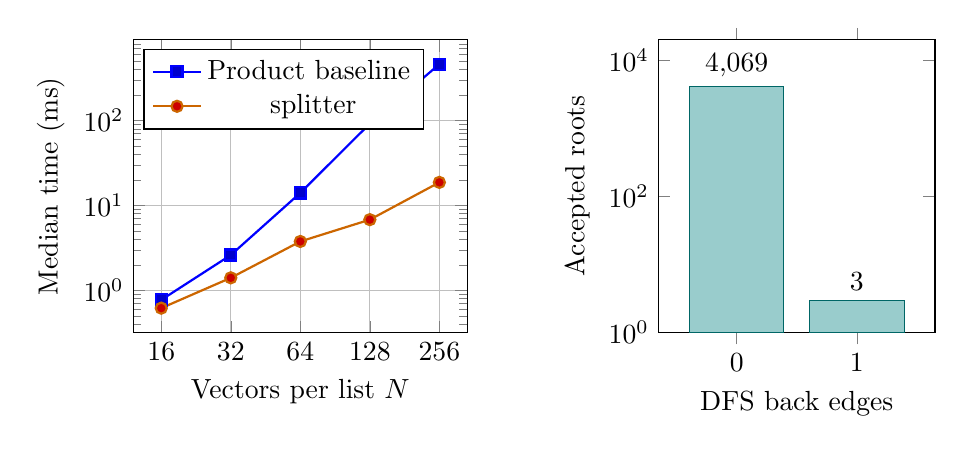
\begin{tikzpicture}
\begin{axis}[width=.48\textwidth,height=53mm,xmode=log,log basis x=2,ymode=log,
 xlabel={Vectors per list $N$},ylabel={Median time (ms)},xtick={16,32,64,128,256},
 xticklabels={16,32,64,128,256},legend pos=north west,legend style={font=\normalsize},
 grid=major,tick label style={font=\normalsize},label style={font=\normalsize}]
\addplot+[mark=square*,blue,thick] coordinates {(16,0.775042) (32,2.613208) (64,14.077417) (128,91.998584) (256,460.842)};
\addlegendentry{Product baseline}
\addplot+[mark=*,orange!80!black,thick] coordinates {(16,0.619833) (32,1.4095) (64,3.776375) (128,6.817959) (256,18.735667)};
\addlegendentry{\musub\ splitter}
\end{axis}
\begin{axis}[at={(.55\textwidth,0)},anchor=south west,width=.42\textwidth,height=53mm,
 ybar,bar width=12mm,ymode=log,ymin=1,ymax=20000,xmin=-.65,xmax=1.65,
 xtick={0,1},xticklabels={0,1},xlabel={DFS back edges},
 ylabel={Accepted roots},ytick={1,100,10000},
 tick label style={font=\normalsize},label style={font=\normalsize},log origin=infty]
\addplot[fill=teal!40,draw=teal!80!black] coordinates {(0,4069)(1,3)};
\node[above,font=\normalsize] at (axis cs:0,4069) {4,069};
\node[above,font=\normalsize] at (axis cs:1,3) {3};
\end{axis}
\end{tikzpicture}
\caption{Left: newly measured times on the compressible synthetic family, including all \musub\ phases. Right: DFS counts only for the $4,072$ extracted corpus roots, or $6.79\%$ of candidates. Both vertical axes are logarithmic.}
\label{fig:experiments}
\end{figure}
